% ---------------- RELAZIONE PROGETTO DI PROGRAMMAZIONE AD OGGETTI (OOP) --------
\documentclass[a4paper,12pt]{report}

% ----------------------------- PREAMBLE --------------------------------------- 

\usepackage{lmodern}
\usepackage{alltt, fancyvrb, url}
\usepackage{float}
\usepackage{graphicx}
\usepackage[utf8]{inputenc}
\usepackage{hyperref}
\usepackage{amsmath,amssymb,amsthm}

\usepackage[italian]{babel}

\usepackage[italian]{cleveref}

\usepackage{comment}
\usepackage{microtype}
\usepackage{fancyhdr}

\usepackage[scaled=.92]{helvet}
\usepackage[T1]{fontenc}

\usepackage{lscape}

\usepackage{subcaption}

% hyperref settings
\hypersetup{
	colorlinks=true,
	linkcolor=black, %blue
	filecolor=magenta,      
	urlcolor=cyan,
	pdftitle={Sharelatex Example},
	bookmarks=true,
	pdfpagemode=FullScreen,
}

\usepackage{titlesec}
%\usepackage{titletoc}

\setcounter{tocdepth}{4}
\setcounter{secnumdepth}{1}

\titleformat{\section}{\normalfont\Large\bfseries\centering}{}{0pt}{} % Questo serve per togliere il numero dalla section

% ----------------------------- PREAMBLE END -----------------------------------

\makeindex

\title{\textbf{Tirocinio} \\[1.5ex] Smart Gardening App}
\author{Luca Rengo}

\begin{document}
	
\makeatletter
\begin{titlepage}
	\begin{center}
		
\includegraphics[width=0.7\linewidth]{images/logo/plant-icon.png}\\
		{\Huge  \@title }\\[3ex] 
		{\large  \@author}\\[3ex] 
		%TODO:
		{\large Maggio | Giugno | Luglio | Agosto | Settembre}\\[3ex]
		{\large 2022}\\[3ex]
	\end{center}
\end{titlepage}
\makeatother
\thispagestyle{empty}
\newpage
	
%\maketitle

\tableofcontents

\newpage

% \input: import the commands from filename.tex to target file.

% \include: does a \clearpage and does an \input.
	
% ============================== INTRODUZIONE =========================================
	
\section{Introduzione}

\textsf{\small L'obiettivo del tirocinio era quello di sviluppare un'applicazione mobile per il monitoraggio della qualità dell'ambiente attraverso dei sensori e la cura delle piante.}

\textsf{\small Il tirocinio si è svolto dal 23-24 maggio ai primi di ottobre 2022.} %TODO: prima era è durato

\begin{comment}
\begin{figure}[ht] 
	\centering
	\includegraphics[width=1.2\textwidth, height=1.2\textheight, keepaspectratio]{./images/}
	\caption{Homepage}
	\label{fig:homepage}
\end{figure}
\end{comment}

% ============================== TECNOLOGIE ===========================================

\section{Tecnologie}

\textsf{\small Le tecnologie utilizzate sono state: \emph{Flutter}, framework per la creazione dell'app, \emph{dart}, il linguaggio del framework, \emph{TensorFlowLite} che è una libreria per il machine learning che ho usato per il riconoscimento delle piante e delle malattie di queste, \emph{Postman} che è un tool per il testing delle API che ho utilizzato per interfacciarmi con le api: \href{open.plantbook.io}{Plantbook} e \href{https://dev.netatmo.com/apidocumentation/oauth}{Netatmo API} attraverso il protocollo standard \emph{OAuth2}.}

% ============================== ATTIVITA' ============================================

\section{Attività}

\textsf{\small Qui, di seguito vado a presentare le varie \emph{features}, sia con tema chiaro che scuro e con lingua italiana e inglese, dell'applicazione: } %TODO: o i vari screens; prima era senza: ", sia con tema chiaro che scuro e con lingua italiana e inglese,"

\subsection{Splash Screen}

\textsf{\small Questo è lo screen di apertura dell'applicazione che dà il benvenuto all'utente.}
\textsf{\small Può essere chiaro o scuro, a seconda del tema selezionato.}

\begin{figure}[H]

\begin{subfigure}{0.3\textwidth}
	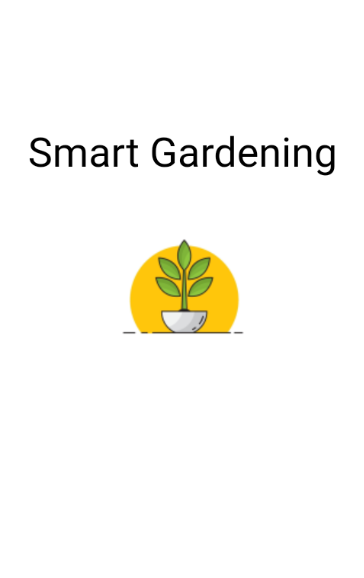
\includegraphics[width=\textwidth]{./images/splash/splash_screen.png}
	\caption{Splash Screen}
	\label{fig:splash_screen}
\end{subfigure}
\hfill
\begin{subfigure}{0.3\textwidth}
	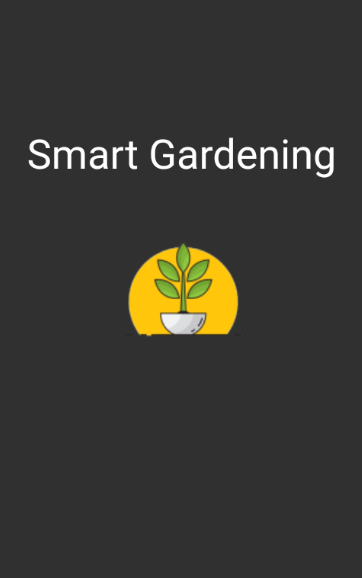
\includegraphics[width=\textwidth]{./images/splash/splash_screen_dark.png}
	\caption{Splash Screen Dark}
	\label{fig:splash_screen_dark}
\end{subfigure}

\end{figure}

\subsection{OnBoarding}

\textsf{\small Dopo lo Splash Screen, c'è una piccola introduzione alle funzionalità dell'app.}

\begin{figure}[H]
	
\begin{subfigure}{0.3\textwidth} %TODO: volendo metterli tutti a 0.2, oppure no, va bene anche così
	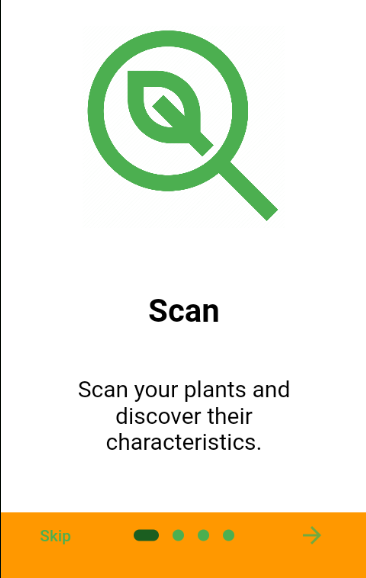
\includegraphics[width=\textwidth]{./images/onboarding/onboarding_screen0.png}
	\caption{OnBoarding Screen Pagina 1}
	\label{fig:onboarding}
\end{subfigure}
\hfill
\begin{subfigure}{0.3\textwidth}
	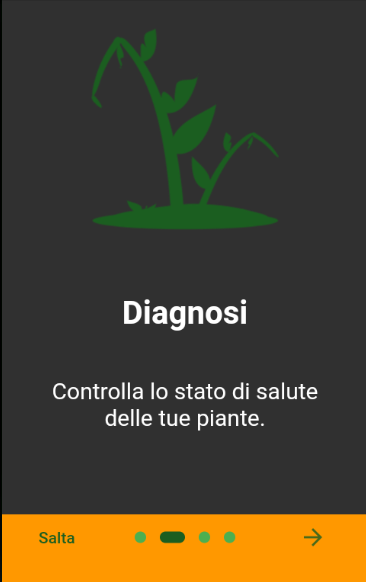
\includegraphics[width=\textwidth]{./images/onboarding/onboarding_screen1_dark.png}
	\caption{OnBoarding Screen Pagina 2}
	\label{fig:onboarding1}
\end{subfigure}
\hfill
\begin{subfigure}{0.3\textwidth}
	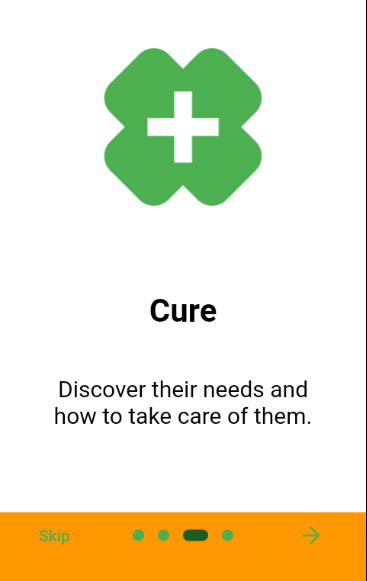
\includegraphics[width=\textwidth]{./images/onboarding/onboarding_screen2.png}
	\caption{OnBoarding Screen Pagina 3}
	\label{fig:onboarding2}
\end{subfigure}
\hfill
\begin{subfigure}{0.3\textwidth}
	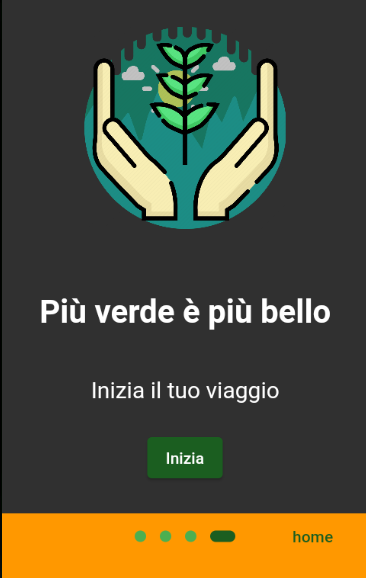
\includegraphics[width=\textwidth]{./images/onboarding/onboarding_screen3_dark.png}
	\caption{OnBoarding Screen Pagina 4}
	\label{fig:onboarding3}
\end{subfigure}
\end{figure}

\subsection{Homepage}

\textsf{\small La Homepage è la pagina principale dell'applicazione, da questa è possibile raggiungere tutte le pagine.}
\textsf{\small In basso è presente una \emph{BottomNavigationBar} che consente un rapido spostamento tra le pagine.}
\textsf{\small In alto a sinistra, cliccando sull'icona menù si potrà accedere al \emph{NavigationDrawer}.}
\textsf{\small In alto a destra, con l'icona della camera, si accede alla schermata della scansione delle piante, mentre con l'icona della bandierina sarà possibile modificare la lingua dell'intera app in tempo reale, senza doverla riavviare.}
\textsf{\small E infine, i pulsanti al centro dello schermo mostrano le varie attività.}

\begin{figure}[ht] 
	\centering
	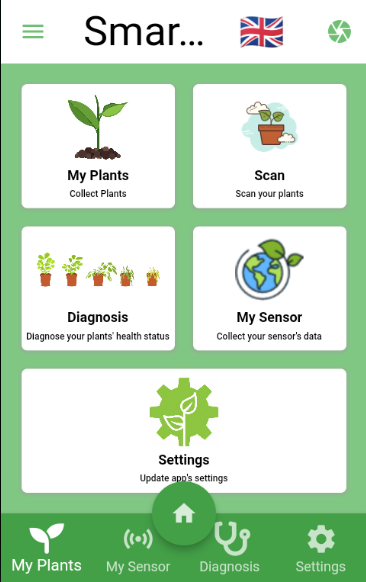
\includegraphics[width=.5\textwidth, height=.5\textheight, keepaspectratio]{./images/home/home_screen.png}
	\caption{Homepage}
	\label{fig:homepage}
\end{figure}
	
% ============================== GUIDA UTENTE =========================================
	
\newpage

\section{Guida utente}

\textsf{\small Qui, di seguito verranno indicate le procedure e le istruzioni da eseguire per poter avviare correttamente l'applicazione: } \\

\begin{itemize}
	\item \textsf{\small }
\end{itemize}

% ============================== CONCLUSIONI ==========================================


\end{document}

% ====================================================================================


